\documentclass[a4paper,11pt]{report}
\usepackage[utf8]{inputenc} % Ac­cept dif­fer­ent in­put en­cod­ings
\usepackage{amsmath} % AMS math­e­mat­i­cal fa­cil­i­ties for LATEX
\usepackage[T1]{fontenc} % Stan­dard pack­age for se­lect­ing font en­cod­ings
\usepackage[portuguese]{babel} % Mul­tilin­gual sup­port for Plain TEX or LATEX
\usepackage{hyperref} % urls
\usepackage{todonotes} % Mark­ing things to do in a LATEX doc­u­ment
\usepackage{bibtopic} % multiples biblios
\usepackage[hang, small,labelfont=bf,up,textfont=it,up]{caption} % Custom captions under/above floats in tables or figures
\usepackage{subfigure}
\usepackage[section]{placeins} % place a \FloatBarrier before every section
\usepackage{algpseudocode} % for algorithms
\usepackage{algorithm} % for algorithms
\usepackage{listings} % for listings
\usepackage{courier} % to show courier when using \texttt or \ttfamily
\usepackage{tikz}
\usetikzlibrary{shapes,arrows,fit,calc,positioning,automata}

% define XOR gate: http://tex.stackexchange.com/questions/75836/creating-a-seamless-xor-symbol-as-node
\tikzset{XOR/.style={draw,circle,append after command={
    [shorten >=\pgflinewidth, shorten <=\pgflinewidth,]
    (\tikzlastnode.north) edge (\tikzlastnode.south)
    (\tikzlastnode.east) edge (\tikzlastnode.west)
}}}

% mudar algorithm para algoritmo
\floatname{algorithm}{Algoritmo}
\renewcommand{\algorithmicrequire}{\textbf{Input:}}
\renewcommand{\algorithmicensure}{\textbf{Output:}}

\numberwithin{algorithm}{section} % Number algorithms within sections (i.e. 1.1, 1.2, 2.1, 2.2 instead of 1, 2, 3, 4)
\numberwithin{equation}{section} % Number equations within sections (i.e. 1.1, 1.2, 2.1, 2.2 instead of 1, 2, 3, 4)
\numberwithin{figure}{section} % Number figures within sections (i.e. 1.1, 1.2, 2.1, 2.2 instead of 1, 2, 3, 4)
\numberwithin{table}{section} % Number tables within sections (i.e. 1.1, 1.2, 2.1, 2.2 instead of 1, 2, 3, 4)
% margins size
\usepackage[margin=2.5cm]{geometry}

\newcommand{\sage}{\textsf{Sage}}

% listings
\definecolor{dkgreen}{rgb}{0,0.6,0}
\definecolor{gray}{rgb}{0.5,0.5,0.5}
\definecolor{mauve}{rgb}{0.58,0,0.82}
\renewcommand{\lstlistingname}{Código}
\lstdefinestyle{Java}{
  frame=tb,
  language=Java,
  tabsize=2,
  breaklines=true,
  breakatwhitespace=true,
  basicstyle=\scriptsize\ttfamily,
  aboveskip=3mm,
  belowskip=3mm,
  numberstyle=\tiny\color{gray},
  captionpos=t,
  extendedchars=true,
  stringstyle=\color{white}\ttfamily,
}
\lstdefinestyle{sage}{
  frame=tb,
  language=Python,
  tabsize=2,
  breaklines=true,
  breakatwhitespace=true,
  basicstyle={\scriptsize\ttfamily},
  aboveskip=3mm,
  belowskip=3mm,
  numberstyle=\tiny\color{gray},
  keywordstyle=\color{blue},
  commentstyle=\color{dkgreen},
  stringstyle=\color{mauve},
  showstringspaces=false,
  captionpos=t,
  %morecomment=[is]{\#}{ } % could be used to hide comments
}

\lstdefinestyle{Bash}{
  language=Bash,
  frame=tb,
  tabsize=2,
  breaklines=true,
  breakatwhitespace=true,
  basicstyle={\scriptsize\ttfamily},
  aboveskip=3mm,
  belowskip=3mm,
  numberstyle=\tiny\color{gray},
  keywordstyle=\color{blue},
  commentstyle=\color{dkgreen},
  stringstyle=\color{mauve},
  showstringspaces=false,
  captionpos=t,
  morekeywords={sage},
  alsoletter={:~$},
  morekeywords=[2]{sage:},
  keywordstyle=[2]{\color{red}},
  literate={\$}{{\textcolor{red}{\$}}}1 
         {:}{{\textcolor{red}{:}}}1
         {~}{{\textcolor{red}{\textasciitilde}}}1,
}

\title{Técnicas Criptográficas -- Exercícios TP}
\author{Nuno Carvalho pg22815 \and Milton Nunes pg22797}
\date{\today}
\begin{document}
\maketitle
\chapter{Grupo I}
O primeiro passo para decifrar os quatro criptogramas é o cálculo do índice de coincidência. A partir desse valor, é possível distinguir entre cifras mono-alfabéticas e poli-alfabéticas, ou em que linguagem se encontra o texto. A fórmula usada para o cálculo do índice de coincidência é a seguinte:
\begin{equation*}
\mathsf{IC} = \dfrac{\sum_{i=0}^{26}{f_i (f_i - 1)}}{n (n - 1)}
\end{equation*}
Sendo $n$ o tamanho do criptograma e $f_i$ a frequência (número de ocorrências) da letra $i$ do alfabeto de 26 letras. Com base nesta fórmula, obtivemos os seguintes valores, sabendo que o \textsf{IC} do inglês e do francês são, respectivamente, 0.0667 e 0.0746:
\begin{itemize}
  \item IC Texto1: 0.0623
  \item IC Texto2: 0.0409
  \item IC Texto3: 0.0799
  \item IC Texto4: 0.0414
\end{itemize}
O texto 1 e o texto 3 parecem ser cifras de substituição mono-alfabética em inglês e francês, respectivamente. O texto 2 e 4 foram provavelmente cifradas com uma cifra de substituição poli-alfabética, nomeadamente com a cifra Vigenère. Ambos são textos em inglês.\\
O texto 1 foi o único que ainda não conseguimos decifrar. De seguida apresentamos os passos dados para cifrar os quatro textos.
\section{Affine}
A chave de uma cifra Affine são dois números $a$ e $b$. A operação de cifração é $E(x) = (ax + b) \pmod{26}$ e a de decifração $D(x) = a^{-1}(x - b) \pmod{26}$, de tal forma que $a$ é coprimo de $m$.\\
Para se atacar a cifra Affine, pode-se usar um método \textit{bruteforce} juntamente com um teste do qui-quadrado para testar a validade da chave obtida. Ou seja, o valor mais baixo do qui-quadrado de todos os candidatos a chave é efectivamente a chave da cifra. Segue-se o código Java para atacar a cifra Affine.
\begin{lstlisting}[style=Java,caption=Método para obter a chave utilizada na cifra Affine.]
public static int[] bruteForceChiSquared(String c, Language l) {
  double smallestChi = -1.0;
  int[] key = new int[2];
  for(int a : Affine.A) { # Affine.A contem todos os coprimos de 26
    for(int b = 0; b < 26; b++) {
      String isM = Affine.dec(a, b, c);
      double chi = Frequencies.chiSquaredStatistic(isM, l);
      if(smallestChi == -1.0) {
        smallestChi = chi;
        key[0] = a; key[1] = b;
      }
      if(chi < smallestChi) {
        smallestChi = chi;
        key[0] = a; key[1] = b;
      }
    }
  }
  return key;
}
\end{lstlisting}
O chave obtida para o texto 3 é $a = 19, b = 4$ e o texto limpo obtido é: \\
\textit{''o canada terre de nos aieux ton front est ceint de fleurons glorieux car ton bras sait porter lepee il sait porter la croix ton histoire est une epopee des plus brillants exploits et ta valeur de foi trempee protegera nos foyers et nos droits''}
\section{Vigenère}
O processo para atacar o Vigenère já não foi tão simples quanto o usado para o Affine. Na nossa abordagem, o primeiro passo foi calcular o tamanho da chave, sabendo que este valor estaria entre dois números não muito grandes (4 a 7). Para o Vigenère, o IC é calculado de forma diferente: pega-se no criptograma, roda-se $x$ posições para a direita e colocam-se ambos os textos em paralelo; o IC é o número de posições onde a mesma letra ocorre tanto no texto original como no texto rodado, a dividir pelo tamanho do criptograma. No nosso caso, o valor de $x$ varia entre 4 e 7. No final, o $x$ cujo IC seja o mais próximo do IC da linguagem é o que representa o tamanho da chave.\\
Tendo o tamanho $d$ da chave, obter a chave torna-se bastante fácil. Basta para isso dividir o texto em $d$ blocos com a forma: para todo o $i$ tal que $1 \leq i \leq d$, $c_i, c_{i+d}, c_{i+2d}, \dotsc$, e sabe-se que cada um destes blocos foi cifrado usando um \textit{shift}. Para descobrir qual o melhor \textit{shift} usa-se a seguinte forma, onde $q_i$ representa a frequência de ocorrências da letra $i$ do alfabeto de 26 letras:
\begin{equation*}
\sum_{i=1}^{26} (q_i - f_i)^2
\end{equation*}
O valor mais pequeno corresponde ao melhor \textit{shift}. No final, a chave é o conjunto dos $d$ melhores \textit{shifts}.\\
A chaves obtidas para os textos 2 e 4 foram, respectivamente, \textsf{crypto} e \textsf{theory}. Os textos limpos são:\\
\textit{''i learned how to calculate the amount of paper needed for a room when i was at school you multiply the square footage of the walls by the cubic contents of the floor and ceiling combined and double it you then allow half the total for openings such as windows and doors then you allow the other half for matching the pattern then you double the whole thing again to give a margin of error and then you order the paper''}\\
\textit{''i grew up among slow talkers men in particular who dropped words a few at a time like beans in a hill and when i got to minneapolis where people took a lake wobegon comma to mean the end of a story i couldnt speak a whole sentence in company and was considered not too bright so i enrolled in a speech course taught by orville sand the founder of reflexive relaxology a self hypnotic technique that enabled a person to speak up to three hundred words per minute''}
\section{Mono-Substituição Alfabética}
O processo utilizado para decifrar o criptograma 1 baseou-se na análise de ocorrência de cada letra do criptograma comparativamente à ocorrência das letras do alfabeto em textos em inglês. Assim, partimos da letra com maior ocorrência, a letra \textit{c}, e substituímos esta pelo \textit{e}. De seguida procuramos a ocorrência dos trigramas mais comuns, acabados em \textit{c}, no criptograma e substituímos pelo trigrama mais comum em inglês \textit{the}. A seguir, substituímos a segunda letra mais frequente do criptograma, \textit{g}, pela letra em inglês mais comum e ainda não utilizada, o \textit{a}. Baseado no \textit{a} procuramos os trigramas mais frequentes começados por esta letra de forma a encontrar ocorrências da palavra \textit{and}. Neste momento, e depois de algumas tentativas de substituição sem sucesso e que não nos levaram a pista nenhuma, verificamos a ocorrência da palavra \textit{dead} que pode indicar que estamos no caminho certo.\\
O resto do processo é semelhante ao descrito até este ponto. A partir dele foram também surgindo partes de palavras que intuitivamente indicam algumas letras a substituir, como \textit{warden} para \textit{garden}, de modo a encontrar o texto limpo. Assim, o texto limpo correspondente ao criptograma 1 é o seguinte:\\
\textit{''i may not be able to grow flowers but my garden produces just as many dead leaves old overshoes pieces of rope and bushels of dead grass as anybodys and today i bought a wheel barrow to help in clearing it up i have always loved and respected the wheel barrow it is the one wheeled vehicle of which i am perfect master''}
%\begin{btSect}{bib/bibz01}
% \section{Bibliografia}
% \btPrintCited
 %\btPrintNotCited
% \btPrintAll
%\end{btSect}

\chapter{Grupo II}
O One-Time Pad é uma cifra que consiste em fazer o XOR do texto limpo com uma chave aleatória do mesmo tamanho que a mensagem a transmitir. Esta cifra, no caso de utilizar uma chave verdadeiramente aleatória e esta se mantiver em segredo torna o criptograma indecifrável, garantido desta forma segurança perfeita. Contudo, no caso de uma chave ser usada mais do que um vez, essa segurança perfeita deixa de existir e a mensagem pode então ser decifrada por um atacante.\\
Assim, se $C_1 = m_1 \oplus k$ e $C_2 = m_2 \oplus k$ e for feita a operação $C_3 = C_1 \oplus C_2$ temos $C_3 = m_1 \oplus m_2$. Desta forma realizamos esta operação para todos os pares possíveis de criptogramas dados. De assinalar que a referida operação de xor neste exercício corresponde à função decifrar.\\
Posto isto, temos um conjunto de novos criptogramas em que um deles deixa de ter uma distribuição de caracteres verdadeiramente aleatória, o que permite que através algumas técnicas usadas em criptoanálise seja possível identificar os criptogramas com maior probabilidade de corresponderem ao que se pretende encontrar. As técnicas que optámos por utilizar foram duas já referidas no guião anterior: Qui-quadrado e o Índice de Coincidência. Os resultados obtidos não foram tal como se esperava muito claros, pois trata-se de um xor entre dois textos limpos apenas composto por letras do alfabeto.\\
Análisamos os resultados obtidos para os 15 criptogramas que apresentam maior probabilidade nas duas técnicas de corresponderem ao criptograma que se pretende descobrir e apenas um é comum a ambas. O criptograma em questão corresponde ao xor dos criptogramas 6 e 18 e apresenta o valor de 878.14 na técnica do Qui-quadrado e de 0.041 relativamente ao Índice de Coincidência. Podemos então concluir que estes dois criptogramas foram muito provavelmente cifrados com a mesma chave. \newline \newline
Em relação ao segundo desafio, optámos, em primeiro lugar, por seguir as mesmas técnicas utilizados no desafio anterior. Contudo verificamos que todos os novos criptogramas apresentam valores semelhantes para o Índice de Coincidência. Posto isto, decidimos analisar a questão da frequência de ocorrência das letras do alfabeto nos criptogramas de forma a podermos encontrar indícios de qual será o criptograma que pretendemos identificar.\\ 
Depois de nos focarmos sobretudo na ocorrência média de cada letra nos criptogramas chegamos a uma conclusão que consideramos poder indicar o criptograma que representa o xor de dois textos limpos.  A nossa teoria baseia-se em fazer a média de ocorrência de cada uma das letras do alfabeto no conjunto dos criptogramas, de seguida para cada criptograma é calculada a diferença de ocorrência de cada letra relativamente à média, a soma das diferenças de cada letra do alfabeto num criptograma dá-nos o que denominamos por desvio.  Esta teoria baseia-se no facto de todos os criptogramas, exceptuando o que é composto pelo xor de dois textos limpos, apresentarem uma distribuição aleatória de letras, assim sendo o criptograma a encontrar será um dos que apresentará um desvio maior relativamente à média, pelo facto de não ter uma distribuição verdadeiramente aleatória. \\
Optámos então por utilizar esta técnica em conjunto com o Qui-quadrado e comparar os resultados obtidos. Assim, tal como no primeiro desafio,  comparando os 15 resultados que apresentam maior probabilidade em cada uma das técnicas, alcançamos 3 resultados em comum: o xor dos criptogramas 5 e 7, 1 e 18 e por fim 17 e 18. Acreditamos então que os criptogramas cifrados com a mesma chave são muito provavelmente um destes três pares. 

\chapter{Grupo III}
\section{Objectivo}
O objectivo principal deste grupo era usar o modo de cifras por blocos ECB em imagens, mais propriamente em imagens que são guardadas como uma matriz de pontos não comprimidas (\textit{bitmap images}). No final, pretendia-se verificar que neste modo é possível retirar informação útil do criptograma, ou seja, é possível verificar certos padrões da imagem original no criptograma.
%
\section{Bitmap image}
Existem vários formatos de \textit{bitmap images}, tais como \textsf{GIF}, \textsf{PNG}, \textsf{TIFF} ou \textsf{JPEG}. Mas nenhum destes formatos serve para o propósito deste grupo, pois são formatos comprimidos. Um outro formato mais conhecido em ambientes \textit{Windows} é o \textsf{BMP}.
Existem várias formas de representar um \verb|BMP|, sendo que é comum a todas elas é o facto de no início do ficheiro estar o cabeçalho. De seguida apresenta-se o formato de um cabeçalho:
\begin{center}
\begin{tabular}{| c | c | p{7cm} |}
  \hline
  \textbf{Posição} & \textbf{Tamanho} & \textbf{Descrição} \\
  \hline
  0x0 & 2 bytes & Serve para identificar o tipo de imagem (normalmente é 0x42 que equivale a \textsf{BMP}) \\
  \hline
  0x2 & 4 bytes & Tamanho do ficheiro em bytes \\
  \hline
  0x6 & 2 bytes & Reservado; depende da aplicação que cria a imagem \\
  \hline
  0x8 & 2 bytes & Reservado; depende da aplicação que cria a imagem \\
  \hline
  0xA & 4 bytes & Indica em que posição começa a matriz de pontos \\
  \hline
\end{tabular}
\end{center}
No âmbito deste trabalho, a informação que mais nos interessa é a posição em que começa a matriz de pontos. Sendo assim, os passos a seguir são:
\begin{enumerate}
  \item Abrir a imagem em modo hexadecimal
  \item Obter a posição onde se encontra a matriz de pontos
  \item Cifrar imagem original em modo ECB
  \item Tendo a imagem cifrada, copiar o conteúdo do cabeçalho da imagem original para o criptograma, caso contrário a imagem não é reconhecida por nenhum leitor de imagens
\end{enumerate}
%
\section{Implementação}
Para se obter o resultado das operações descritas anteriormente, são fundamentalmente precisas três ferramentas:
\begin{description}
  \item[od] Para abrir um ficheiro em modo hexadecimal, podendo assim manipulá-lo \textit{byte} a \textit{byte}
  \item[OpenSSL] Para cifrar a imagem em modo ECB
  \item[dd] Para copiar certas quantidades de \textit{bytes} de um ficheiro para outro
\end{description}
Estas três ferramentas são combinadas entre si usando vários comandos \textsf{Bash} tais como \verb|head|, \verb|tail| ou o redireccionamento de \textit{streams}.\\
Para se obter a posição inicial da matriz de pontos, usa-se o seguinte comando:
\begin{lstlisting}[style=Bash]
od -t x -An $IFILE  | head -n1 | cut -d' ' -f4,5 | tr -d ' ' | tail -c15 | cut -c1-8
\end{lstlisting}
De seguida explica-se o que cada um dos comandos faz:
\begin{description}
  \item[od -t x -An] lê todo o ficheiro \verb|$IFILE| em modo hexadecimal
  \item[head -n1] apresenta apenas a primeira linha do ficheiro; essa primeira linha contém os primeiros 16 \textit{bytes} do ficheiro, representados por 4 blocos de 4 \textit{bytes}. Vamos usar os seguintes 16 \textit{bytes} como exemplo a partir de agora: \verb|687a4d42 00000010 007a0000 006c0000|
  \item[cut -d' ' -f4,5] para se obterem os terceiro e quarto blocos de \textit{bytes}. No exemplo, obtém-se \verb|007a0000 006c0000|
  \item[tr -d ' '] apagar os espaços em branco. Fica-se com \verb|007a0000006c0000|
  \item[tail -c15] obtem os últimos 15 caractéres (ou seja, 7 \textit{bytes} e um \verb|\n|). Fica-se com \verb|7a0000006c0000|
  \item[cut -c1-8] obtem os primeiros 8 caractéres, ou seja, 4 \textit{bytes}. Fica-se com \verb|7a000000|
\end{description}
O resultado obtido anteriormente está no formato \textit{little endian}, ou seja, é necessário convertê-lo para \textit{big endian}, para depois o converter para decimal. Eis como o fizemos no nosso script, estando em \verb|$HEADERSIZE_LE| o resultado anterior \verb|7a000000|:
\begin{lstlisting}[style=Bash]
HEADERSIZE=""
for (( i = 0; i < ${#HEADERSIZE_LE}; i+=2 )); do
  BYTE=${HEADERSIZE_LE:$i:2} # get substring starting in $i with 2 chars
  HEADERSIZE=$BYTE$HEADERSIZE
done
# convert header size to decimal
HEADERSIZE=$(echo "obase=10; ibase=16; $HEADERSIZE" | bc)
\end{lstlisting}
No exemplo anterior, o valor de \verb|HEADERSIZE| é 122.\\
Nesta altura, já podemos cifrar a matriz de pontos. Para isso usamos o \textsf{dd} para obter e cifrar apenas os \textit{bytes} necessários.\\
Em primeiro lugar, copiámos apenas o \textit{header} da imagem original para o ficheiro de destino \verb|OFILE|.
\begin{lstlisting}[style=bash]
dd if="$IFILE" of="$OFILE" bs=1 count="$HEADERSIZE" conv=notrunc 2> /dev/null
\end{lstlisting}
De seguida, ciframos a matriz de pontos e redireccionámos o resultado para o ficheiro de destino. A matriz de pontos de pontos é lida directamente a partir do ficheiro original, usando também o \textsf{dd}, e o seu resultado é enviado através do \textsf{stdin} para o \textsf{OpenSSL}.
\begin{lstlisting}[style=bash]
dd if="$IFILE" bs=1 skip="$HEADERSIZE" conv=notrunc 2> /dev/null | openssl enc -e "$CIPHER" >> "$OFILE"
\end{lstlisting}
De forma a automatizar este processo, criou-se um pequeno \textit{script} em \textsf{Bash}. O Código~\ref{ecb:script} e a sua invocação é a seguinte:
\begin{lstlisting}[style=Bash]
$ ./script infile.bmp outfile.bmp ecb-cipher
$ ./script car.bmp car-des.bmp -des-ecb
\end{lstlisting}
\begin{lstlisting}[style=Bash,caption={\textit{Script} utilizado para cifrar imagens com uma cifra por blocos.},label=ecb:script]
#!/bin/bash

usage() {
  echo "Chamaste mal o script"
  exit
}

if [ -z "$1" ] || [ -z "$2" ] || [ -z "$3" ]; then
  usage
fi
IFILE="$1"
if [ ! -f "$IFILE" ]; then
  echo $IFILE" does not exist."
  exit
fi
OFILE="$2"
if [ -f "$OFILE" ]; then
  echo $OFILE" already exists. Cannot proceed"
  exit
fi
CIPHER="$3"

HEADERSIZE_LE=$(od -t x -An "$IFILE" | head -n1 | \
  cut -d' ' -f4,5 | tr -d ' ' | tail -c15 | cut -c1-8)
HEADERSIZE_LE="${HEADERSIZE_LE^^}"

HEADERSIZE=""
for (( i = 0; i < ${#HEADERSIZE_LE}; i+=2 )); do
  BYTE=${HEADERSIZE_LE:$i:2}
  HEADERSIZE=$BYTE$HEADERSIZE
done
HEADERSIZE=$(echo "obase=10; ibase=16; $HEADERSIZE" | bc)
echo "Header size of '"$IFILE"' is "$HEADERSIZE" bytes, located at position 0x0A"

dd if="$IFILE" of="$OFILE" bs=1 count="$HEADERSIZE" \
  conv=notrunc 2> /dev/null

dd if="$IFILE" bs=1 skip="$HEADERSIZE" \
  conv=notrunc 2> /dev/null | \
  openssl enc -e "$CIPHER" >> "$OFILE"
\end{lstlisting}
\section{Exemplos e conclusões}
Decidimos usar como exemplos as seguintes imagens:
\begin{figure}[htb]
\centering
\subfigure[Famosa imagem do pinguim]{
\includegraphics[scale=0.45, keepaspectratio = true]{img/penguin}}
\subfigure[Carro]{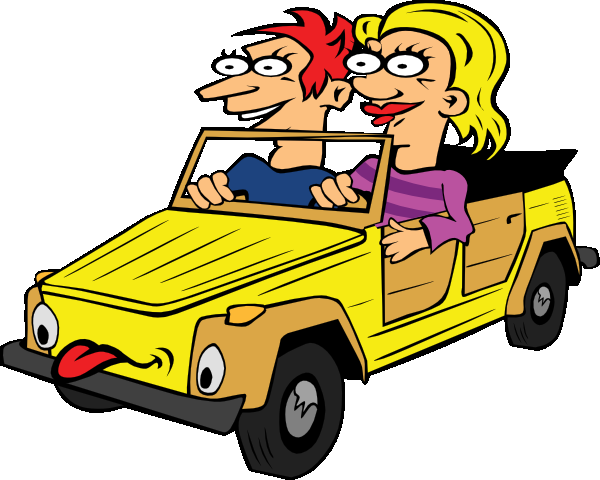
\includegraphics[scale=0.35, keepaspectratio = true]{img/car}}
\caption{Exemplos utilizados}
\end{figure}
Vamos cifrar com DES e com AES para ver se existem diferenças claras entre ambas. Em todas elas, a \textit{passphrase} utilizada é \textsf{passphrase-quase-quase-boa-para-usar-com-o-modo-ecb}.\\
Cifrando com o DES e AES, obtêm-se os seguintes resultados:
\begin{figure}[htb]
\centering
\subfigure[Pinguim, utilizando o comando \texttt{./script penguin.bmp penguin-des.bmp -des-ecb}]{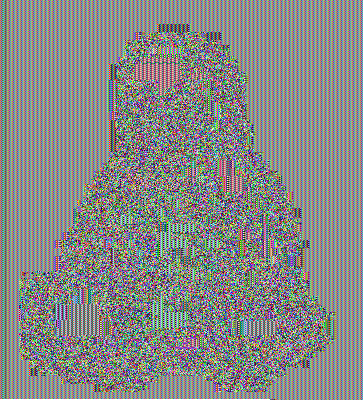
\includegraphics[scale=0.45, keepaspectratio = true]{img/penguin-des}}
\subfigure[Carro, utilizando o comando \texttt{./script car.bmp car-des.bmp -des-ecb}]{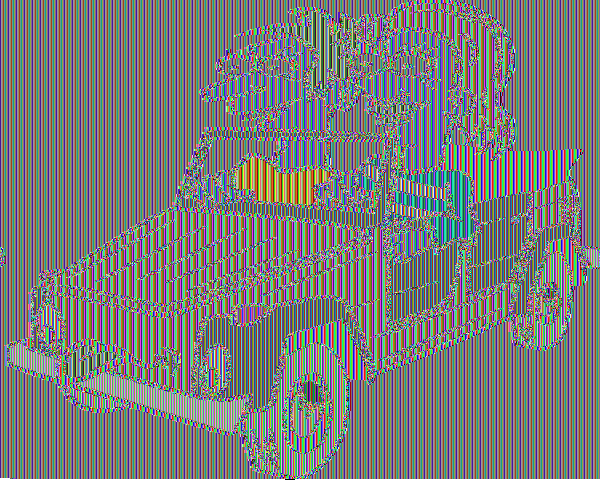
\includegraphics[scale=0.35, keepaspectratio = true]{img/car-des}}
\caption{Cifração com DES em modo ECB}
\end{figure}
%
\begin{figure}[htb]
\centering
\subfigure[Pinguim, utilizando o comando \texttt{./script penguin.bmp penguin-aes192.bmp -aes-192-ecb}]{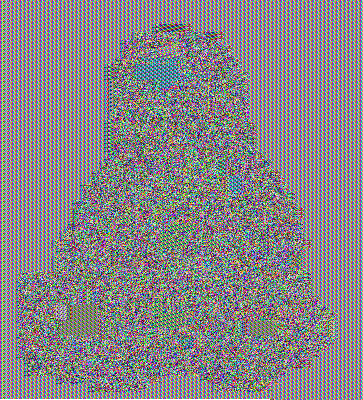
\includegraphics[scale=0.45, keepaspectratio = true]{img/penguin-aes192}}
\subfigure[Pinguim, utilizando o comando \texttt{./script penguin.bmp penguin-aes192.bmp -aes-192-ecb}]{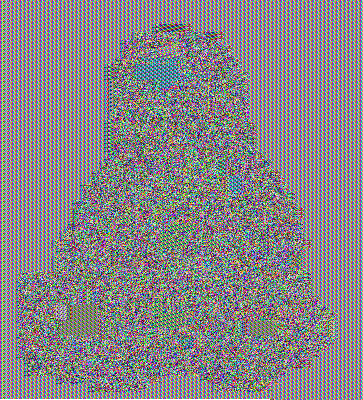
\includegraphics[scale=0.45, keepaspectratio = true]{img/penguin-aes192}}
\subfigure[Carro, utilizando o comando \texttt{./script car.bmp car-aes192.bmp -aes-256-ecb}]{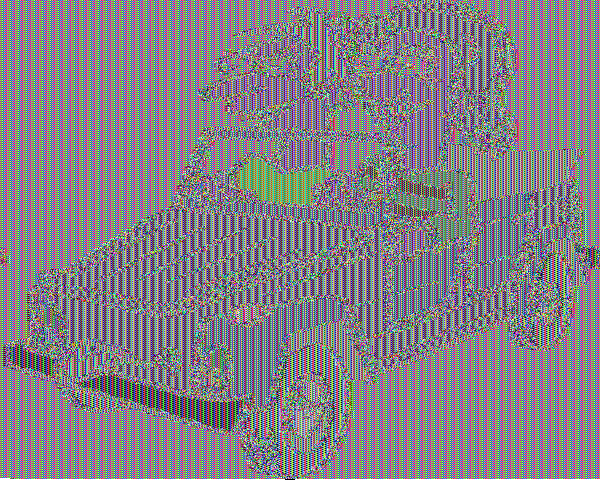
\includegraphics[scale=0.35, keepaspectratio = true]{img/car-aes256}}
\subfigure[Carro, utilizando o comando \texttt{./script car.bmp car-aes192.bmp -aes-256-ecb}]{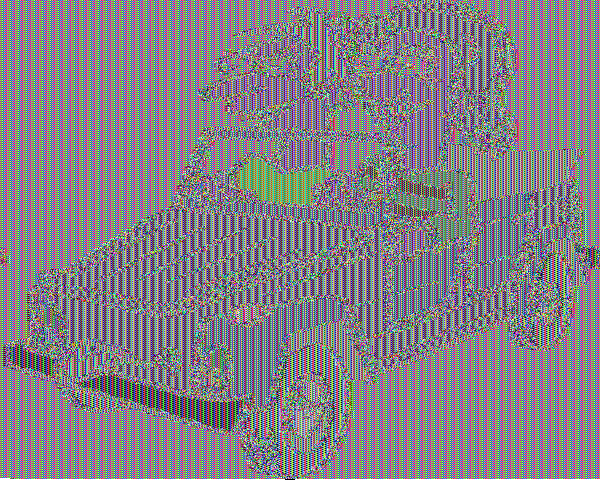
\includegraphics[scale=0.35, keepaspectratio = true]{img/car-aes256}}
\caption{Cifração com AES em modo ECB, com 192 e 256 bits}
\end{figure}
%
Como se pode ver, não existe uma diferença clara entre o AES e o DES. Da mesma forma, também não existe nenhuma diferença entre o AES com 192 e 256 bits. No entanto, é claro que em todas as cifras, em conjunto com o ECB, é possível encontrar certos padrões da mensagem original.
%
%\begin{btSect}{bib/bibz03}
% \section{Bibliografia}
 %\btPrintCited
 %\btPrintNotCited
% \btPrintAll
%\end{btSect}
\chapter{Grupo IV}
\section{Implementação}
A implementação do CBC-MAC em \sage\ é bastante simples. Usa-se como função pseudo-aleatória a cifra por blocos AES, através da biblioteca \verb|pycrypto|. Vamos usar como valores \textit{default} chaves de $n = 128$ bits e $\ell(n) = 5$, ou seja, mensagens de comprimento $640$ bits ($80$ caractéres) divididas em blocos de $128$ bits ($16$ caractéres). Considerem-se a mensagem $m = m_1\ ||\ m_2\ ||\ \cdots\ ||\ m_{\ell(n)}$, com as \textit{tags} $t = t_1\ ||\ t_2\ ||\ \cdots\ ||\ t_{\ell(n)}$ ($\mathsf{Mac_k}(m)$ apenas retorna o bloco $t_{\ell(n)}$).
%%%%% Return all blocks
\section{Retornar todos os blocos}
Retornar todos os blocos da \textit{tag} torna o CBC-MAC inseguro pois torna-se bastante fácil falsificar MAC's. Na imagem~\ref{img:cbcmac} é demonstrado o mecanismo de falsificação de MAC's para uma mensagem em que é criada uma mensagem falsa $m' =  (t_1 \oplus m_2)\ ||\ m_3\ ||\ \cdots\ ||\ m_\ell(n)\ ||\ (t_{\ell(n)} \oplus m_1)$. A \textit{tag} usada para verificação é apenas $t_{\ell(n)}$.
\begin{figure}[h!]
\centering
  \tikzset{line/.style={draw, -latex',shorten <=1bp,shorten >=1bp}}

\begin{tikzpicture}
  %\draw[help lines] (0,0) grid (9, 9);
  \foreach \i in {0,...,2} { %%% CHANGE NUMBER OF BLOCKS HERE! %%%
    \pgfmathsetmacro{\z}{3.5*\i}
    % draw k
    \node (k\i) at (-0.5 + \z, 2) {\textsf{k}};
    % draw box
    \path[draw] (0.5 + \z, 1.5) -- ++(1.5, 0) -- ++(0, 1) -- ++(-1.5, 0) -- ++(0, -1);
    % draw text
    \node (F\i) at (1.25 + \z, 2) {$\mathsf{F_k}$};
    % this macros cast the float to integer
    \pgfmathtruncatemacro{\t}{1+\i}
    \pgfmathtruncatemacro{\m}{2+\i}
    \pgfmathtruncatemacro{\r}{4 - \i} %%% CHANGE NUMBER OF BLOCKS HERE! %%%
    %%%% if \i != 0 %%%%
    \ifthenelse{\NOT 0 = \i} {
      % draw XOR gate in all blocks, except the first
      \node (XOR\i)[XOR] at (1.25 + \z, 3.75) {};
      % draw arrows above F_k
      \path[line] (XOR\i) edge ++(0, -1.25) % xor to F_k
                  (k\i) edge ++(1, 0); % k to F_k
      %%%% last block %%%%
      \ifthenelse{2 = \i}{ %%% CHANGE NUMBER OF BLOCKS HERE! %%%
        % draw input block
        \node (m\i) at (1.25 + \z, 5) {$t_{\ell(n)} \oplus m_{1}$};
        % draw output block
        \node (t\i) at (1.25 + \z, 0) {$t_{\ell(n)}$};
      }
      %%%% all blocks, except first and last %%%%
      {
        % draw input block
        \node (m\i) at (1.25 + \z, 5) {$m_{\r}$};
        % draw output block
        \node (t\i) at (1.25 + \z, 0) {$t_{\m}$};
      }
      % draw arrows above F_k
      \path[line] (m\i) edge (XOR\i); % input block to xor
    }
    %%%% first block %%%%
    {
      % draw input block
      \node (m\i) at (1.25 + \z, 5) {$t_{\t} \oplus m_{\m}$};
      % draw arrows above F_k
      \path[line] (m\i) edge ++(0, -2.5) % input block to F_k
                  (k\i) edge ++(1, 0); % k to F_k
      % draw output block
      \node (t\i) at (1.25 + \z, 0) {$t_{\m}$};
      
    }
    % dont add padding to the beggining of the line
    %\tikzset{line/.style={draw, -latex',shorten <=0bp,shorten >=1bp}}
    \path[line] (1.25 + \z, 1.5) -- (t\i); % F_k box to block
    %\tikzset{line/.style={draw, -latex',shorten <=1bp,shorten >=1bp}}
  }
  
  %%%% draw only arrows
  \foreach \i in {0,...,2} { %%% CHANGE NUMBER OF BLOCKS HERE! %%%
    \pgfmathsetmacro{\z}{3.5*\i}
    \pgfmathtruncatemacro{\t}{1+\i}
    \pgfmathtruncatemacro{\u}{1-\i}
    \ifthenelse{\NOT 2 = \i} { %%% CHANGE NUMBER OF BLOCKS HERE! %%%
      \ifthenelse{1 = \i}{  %%% CHANGE NUMBER OF BLOCKS HERE! %%%
        \node (dots1) at (3 + \z, 5) {$\cdots$};
        \node (dots1) at (3 + \z, 3.25) {$\cdots$};
        \node (dots1) at (3 + \z, 0) {$\cdots$};
        \path[line] (4 + \z, 3.75) -- (XOR\t);
      }
      {
        % draw arrow from F_k to XOR
        \path[line] (1.25 + \z, 1) -- ++(1.25, 0) -- ++(0, 2.75) -- (XOR\t);
      }
    }
    {
    }
    
  }

  % dont add padding to the beggining of the line
  \tikzset{line/.style={draw, -latex',shorten <=0bp,shorten >=1bp}}
  %\path[line] (3, 4) -- (t1XORm3);
\end{tikzpicture}
  \caption{Falsificação de MAC's quando todos os blocos da \textit{tag} são retornados por \textsf{Mac}.}
  \label{img:cbcmac}
\end{figure}
%
%%%%%% Use random IV
\section{Usar um \textsf{IV} aleatório}
Usando um \textsf{IV} aleatório $iv$ ainda se torna mais fácil falsificar mensagens (sendo que \textsf{Mac} apenas retorna o último bloco como \textit{tag}). Basta para isso criar a nova mensagem $m' = (m_1 \oplus iv)\ ||\ m_2\ ||\ \cdots\ ||\ m_{\ell(n)}$ e a tag $t' = t$ tal que $\mathsf{Vrfy_k}(m', t') = \top$.
\begin{figure}[h!]
\centering
  \tikzset{line/.style={draw, -latex',shorten <=1bp,shorten >=1bp}}

\begin{tikzpicture}
  %\draw[help lines] (0,0) grid (9, 9);
  \foreach \i in {0,...,2} { %%% CHANGE NUMBER OF BLOCKS HERE! %%%
    \pgfmathsetmacro{\z}{3.5*\i}
    % draw k
    \node (k\i) at (-0.5 + \z, 2) {\textsf{k}};
    % draw box
    \path[draw] (0.5 + \z, 1.5) -- ++(1.5, 0) -- ++(0, 1) -- ++(-1.5, 0) -- ++(0, -1);
    % draw text
    \node (F\i) at (1.25 + \z, 2) {$\mathsf{F_k}$};
    % this macros cast the float to integer
    \pgfmathtruncatemacro{\t}{1+\i}
    \pgfmathtruncatemacro{\m}{2+\i}
    \pgfmathtruncatemacro{\r}{4 - \i} %%% CHANGE NUMBER OF BLOCKS HERE! %%%
    %%%% if \i != 0 %%%%
    \ifthenelse{\NOT 0 = \i} {
      % draw XOR gate in all blocks, except the first
      \node (XOR\i)[XOR] at (1.25 + \z, 3.75) {};
      % draw arrows above F_k
      \path[line] (XOR\i) edge ++(0, -1.25) % xor to F_k
                  (k\i) edge ++(1, 0); % k to F_k
      %%%% last block %%%%
      \ifthenelse{2 = \i}{ %%% CHANGE NUMBER OF BLOCKS HERE! %%%
        % draw input block
        \node (m\i) at (1.25 + \z, 5) {$m_{\ell(n)}$};
        % draw output block
        \node (t\i) at (1.25 + \z, 0) {$t_{\ell(n)}$};
      }
      %%%% all blocks, except first and last %%%%
      {
        % draw input block
        \node (m\i) at (1.25 + \z, 5) {$m_{\t}$};
        % draw output block
        \node (t\i) at (1.25 + \z, 0) {$t_{\t}$};
      }
      % draw arrows above F_k
      \path[line] (m\i) edge (XOR\i); % input block to xor
    }
    %%%% first block %%%%
    {
      % draw input block
      \node (m\i) at (1.25 + \z, 5) {$m_{\t} \oplus iv$};
      % draw arrows above F_k
      \path[line] (m\i) edge ++(0, -2.5) % input block to F_k
                  (k\i) edge ++(1, 0); % k to F_k
      % draw output block
      \node (t\i) at (1.25 + \z, 0) {$t_1$};
      
    }
    % dont add padding to the beggining of the line
    %\tikzset{line/.style={draw, -latex',shorten <=0bp,shorten >=1bp}}
    \path[line] (1.25 + \z, 1.5) -- (t\i); % F_k box to block
    %\tikzset{line/.style={draw, -latex',shorten <=1bp,shorten >=1bp}}
  }
  
  %%%% draw only arrows
  \foreach \i in {0,...,2} { %%% CHANGE NUMBER OF BLOCKS HERE! %%%
    \pgfmathsetmacro{\z}{3.5*\i}
    \pgfmathtruncatemacro{\t}{1+\i}
    \pgfmathtruncatemacro{\u}{1-\i}
    \ifthenelse{\NOT 2 = \i} { %%% CHANGE NUMBER OF BLOCKS HERE! %%%
      \ifthenelse{1 = \i}{  %%% CHANGE NUMBER OF BLOCKS HERE! %%%
        \node (dots1) at (3 + \z, 5) {$\cdots$};
        \node (dots1) at (3 + \z, 3.25) {$\cdots$};
        \node (dots1) at (3 + \z, 0) {$\cdots$};
        \path[line] (4 + \z, 3.75) -- (XOR\t);
      }
      {
        % draw arrow from F_k to XOR
        \path[line] (1.25 + \z, 1) -- ++(1.25, 0) -- ++(0, 2.75) -- (XOR\t);
      }
    }
    {
    }
    
  }

  % dont add padding to the beggining of the line
  \tikzset{line/.style={draw, -latex',shorten <=0bp,shorten >=1bp}}
  %\path[line] (3, 4) -- (t1XORm3);
\end{tikzpicture}
  \caption{Falsificação de MAC's quando se utiliza um \textsf{IV} aleatório.}
  \label{img:randiv}
\end{figure}
%%%% exemplo ataque
\section{Implementação e execução \sage}
Depois de implementado o CBC-MAC, criaram-se dois métodos na classe \verb|CBCMAC| para falsificar mensagens:
\begin{description}
  \item[ForgeMacRandomIV(msg, tag, iv)] Retorna o par $(msg', tag)$
  \item[ForgeMacAllTags(msg, tag)] Retorna o par $(msg', tag')$
\end{description}
Além disso, o método \textsf{Mac} tem uma variante insegura, bastante para isso incluir o argumento \verb|secure=False| na sua invocação.\\
Segue-se o exemplo de uma sessão \sage\ em que se falsificam algumas mensagens.
\begin{lstlisting}[style=Bash,caption=Exemplo de falsificação de MACs em \sage]
sage: CBC = CBCMAC(128,5)
sage: key = MyKey(length=128)
sage: m = 'Isto e o CBC-MAC. Vamos forgar esta mensagem usando dois metodos. Wish me luck!!'
sage: iv = randomIV()
sage: t = CBC.Mac(key, m, iv=iv) # auth msg using random IV
sage: (m2, t2) = CBC.ForgeMacRandomIV(m, t, iv) # forge new msg and tag
sage: CBC.Vrfy(key, m, t, iv) # Vrfy using the random IV
True
sage: m2 ; CBC.Vrfy(key, m2, t2)
'<\xd0w\xc2#\xc6\xdaa[\x8eH\x94\x0el0\xb2. Vamos forgar esta mensagem usando dois metodos. Wish me luck!!'
True
sage: CBC.Vrfy(key, m, t) # Vrfy using IV = 0
False
sage: (iv,t) = CBC.Mac(key, m, secure=False) # auth msg and return all blocks
sage: (m3, t3) = CBC.ForgeMacAllTags(m, t) # forge new msg and tag
sage: m3 ; CBC.Vrfy(key, m3, t3) # Vrfy new forged msg
'\xad\x11q\xe0X IG\xf8\xd4\x1c\x10\x10\x85\xfaMsta mensagem usando dois metodos. Wish me luck!!\x0f\xdd0\x9fh=I\xdbB=\x8f"g\x88\x00\x96'
True
\end{lstlisting}
%\begin{btSect}{bib/bibz04}
% \section{Bibliografia}
 %\btPrintCited
 %\btPrintNotCited
% \btPrintAll
%\end{btSect}

\chapter{Grupo V}
\section{Congruências}
Para resolver os sistemas de congruências podemos utilizar o Teorema Chinês dos Restos (CRT). O CRT serve exactamente para resolver os sistemas de congruências dados no enunciado, ou seja, tendo um conjunto $n_1, \dotsc, n_k$ de inteiros mutualmente coprimos e dada uma sequência de inteiros $a_1, \dotsc, a_k$, existe um inteiro $x$ que resolve o seguinte sistema de congruências:
\begin{equation*}
\begin{matrix}
x \equiv a_1 \pmod{n_1} \\
x \equiv a_2 \pmod{n_2} \\
\vdots                  \\
x \equiv a_k \pmod{n_k} \\
\end{matrix}
\end{equation*}
Para calcular o CRT precisamos de utilizar o algoritmo de Euclides estendido. Com o Euclides estendido (\textsf{extendedgcd}) podemos encontrar os inteiros $r_i$ e $s_i$ tal que $r_i n_i + s_i (N/n_i) = 1$. Ambos os algoritmos são apresentados em \ref{alg:xgcd} e \ref{alg:crt}.\\
\begin{algorithm}
  \caption{Algoritmo de Euclides estendido}\label{alg:xgcd}
  \begin{algorithmic}
    \Require Inteiros $a \geq b > 0$
    \Ensure $(g, X, Y)$ com $g = \gcd{(a,b)}$ e $g = Xa + Yb$
    \State $x \gets 0, y \gets 1$
    \State $lastx \gets 1, lasty \gets 0$
    \While{$b \neq 0$}
      \State $quot \gets a \text{ div } b$
      \State $(a,b) \gets (b, a \bmod b)$
      \State $(x, lastx) \gets (lastx - quot \times x, x)$
      \State $(y, lasty) \gets (lasty - quot \times y, y)$
    \EndWhile
    \State $g \gets (lastx \times a_{pre}) + (lasty \times b_{pre})$
    \Comment{$a_{pre}$ e $b_{pre}$ valores originais de $a$ e $b$}
    \State \Return $(g, lastx, lasty)$
  \end{algorithmic}
\end{algorithm}
%
\begin{algorithm}
  \caption{Teorema Chinês dos Restos}\label{alg:crt}
  \begin{algorithmic}
    \Require $x \equiv a_i \pmod{n_i}\ \text{para } i = 1, \dotsc, k$ tal que $n_i$ e $N/n_i$ são coprimos
    \Ensure $x$ tal que resolve o sistema de congruências
    \State $N \gets \prod_{i = 1}^k{n_i}$
    \State $x \gets 0$
    \For{$i = 1$ to $k$}
      \State $(g, r_i, s_i) \gets \mathsf{extendedgcd}(n_i, N/n_i)$
      \Comment{verifica-se sempre $g = 1$}
      \State $e_i \gets s_i \times (N/n_i)$
      \State $x \gets x + a_i \times e_i$
    \EndFor
    \State \Return $x \bmod{N}$
  \end{algorithmic}
\end{algorithm}
Optámos por implementar os algoritmos em \sage, sendo o~\ref{alg:xgcd} implementado como \verb|extended_gcd(a, b)| e o CRT como \verb|solve_congruences(a, n)|. Note-se que os parâmetros \verb|a| e \verb|n| de \verb|solve_congruences| deverão ser listas inteiros de igual comprimento.\\
Usando a função \verb|solve_congruences|, é bastante simples resolver os dois primeiros exercícios deste grupo. Mas para resolver o segundo exercício, é preciso chegar à seguinte conclusão:
\begin{equation*}
\left\{
  \begin{array}{l l}
    13x \equiv 4  \pmod{99}  \\
    15x \equiv 56 \pmod{101} \\
  \end{array}
\right.
\Leftrightarrow
\left\{
  \begin{array}{l l}
    x \equiv 4/13  \pmod{99}  \\
    x \equiv 56/15 \pmod{101} \\
  \end{array}
\right.
\Leftrightarrow
\left\{
  \begin{array}{l l}
    x \equiv 46  \pmod{99} \\
    x \equiv 98 \pmod{101} \\
  \end{array}
\right.
\end{equation*}
em que $\bmod{(4/13, 99)} = 46$ e $\bmod{(56/15, 101)} = 98$.\\
Sendo assim, basta executar os seguintes comandos em \sage:
\scriptsize\begin{verbatim}
sage: solve_congruences([12, 9, 23], [25, 26, 27])
14387
sage: solve_congruences([46, 98], [99, 101])
7471
\end{verbatim}\normalsize
\section{RSA}
São nos dadas duas chaves públicas com módulos $n$ pequenos e de fácil factorização. Logo, para decifrar os textos basta:
\begin{enumerate}
  \item factorizar $n$ para obter o os factores $p \cdot q = n$
  \item calcular $\phi(n) = (p-1)(q-1)$
  \item calcular expoente privado $d$ tal que $d^{-1} \equiv e \pmod{\phi(n)}$. Neste momento, temos a chave privada e podemos decifrar os textos
  \item decifrar os textos número a número, ou seja, decifra-se um número de cada vez para se obter o trio de letras original
  \item concatenar os resultados obtidos para criar o texto original
\end{enumerate}
\subsection{Factorizar $n$}
Dado que, como referido, a factorização é feita sobre $n$ pequenos a função de factorização é bastante simples:
\begin{lstlisting}[style=sage]
def factorN(n):
  for i in range(5, 500):
    for j in range(5, 500):
      if i*j == n:
        return (i,j)
  return -1
\end{lstlisting}
\subsection{Cálculo expoente privado $d$}
Para calcular o expoente privado $d$ é, em primeiro lugar calculado o valor de $\phi(n)$:
\begin{lstlisting}[style=sage]
 phi = (p-1)*(q-1)
\end{lstlisting}
De assinalar que $p$ e $q$ são o resultado da função de factorização de $n$. De seguida, é então calculado o expoente privado:
\begin{lstlisting}[style=sage]
 d = Integer(e).inverse_mod(phi)
\end{lstlisting}
\subsection{Decifração e descodificação}\label{subsec:decode}
De forma a recuperar o texto limpo foram desenvolvidas as seguintes funções que permitem decifrar e descodificar os criptogramas dados:
\begin{lstlisting}[style=sage]
def dec(sk, c):
  return power_mod(c, sk[1], sk[0])

def decText(sk, text):
  return ''.join(map(lambda x : decodeTri(dec(sk, x)) , text))

def intToChr(i):
  return abc[i]

def decodeTri(t):
  for i in xrange(0,26):
    for j in xrange(0,26):
      for k in xrange(0,26):
        if ((i*(26**2)) + (j*26) + k) == t:
          return str(intToChr(i) + intToChr(j) + intToChr(k))
\end{lstlisting}
Assim foi possível recuperar textos limpos dos criptogramas 1 e 2 indicados no enunciado, respectivamente:\\
\textit{''lake wobegon is mostly poor sandy soil and every spring the earth heaves up a new crop of rocks piles of rocks ten feet high in the corners of fields picked by generations of us monuments to our industry our ancestors chose the place tired from their long journey sad for having left the mother land behind and this place reminded them of there so they settled here forgetting that they had left there because the land wasnt so good so the new life turned out to be a lot like the old except the winters are worsez''} \\
\textit{''i became involved in an argument about modern painting a subject upon which i am spectacularly ill informed however many of my friends can become heated and even violent on the subject and i enjoy their wrangles in a modest way i am an artist myself and i have some sympathy with the abstractionists although i have gone beyond them in my own approach to art i am a lumpist two or three decades ago it was quite fashionable to be a cubist and to draw every thing in cubes then there was a revolt by the vorticists who drew every thing in whirls we now have the abstractionists who paint every thing in a very abstracted manner but my own small works done on my telephone pad are composed of carefully shaded strangely shaped lumps with traces of cubism vorticism and abstractionism in them for those who possess the seeing eye as a lumpist i stand alone''}
\section{Calcular Símbolos de Jacobi}
Os Símbolos de Jacobi, que consistem numa generalização dos Símbolos de Legendre, foram criados por Jacobi em 1837 e revelaram-se bastante úteis em vários ramos da teoria dos números, especialmente na teoria computacional dos números, nomeadamente no teste de primalidade e factorização de inteiros, e portanto também muito importantes em criptografia.\\
De forma a ser possível calcular os Símbolos de Jacobi e testar o programa para os \textit{inputs} dados foi desenvolvida em \textit{Sage} uma função recursiva que implementa as quatro propriedades pretendidas. Abaixo é apresentado o código desenvolvido:
\begin{lstlisting}[style=sage]
def jacobi(m,n):
  if not is_odd(n):
    print "n not odd"
    return
  if m == 0:
    return 0
  if m == 1:
    return 1
  #propriedade a)
  if m>=n:
    return jacobi(m%n, n)
  #propriedade b)
  if m == 2:
    nm8 = n%8
    if nm8 == 1.mod(8) or nm8 == (-1).mod(8):
      return 1
    elif nm8 == 3.mod(8) or nm8 == (-3).mod(8):
      return -1
  #propriedade c)
  f = list(factor(m))
  if len(f) == 2 and f[1][1] == 1 and f[0][0] == 2:
    return ((jacobi(2, n)**f[0][1]))*jacobi(f[0][1], n)
  if m%2 == 0:
    return jacobi(2,n)*jacobi(m//2,n)
  #propriedade d)
  if m%4 == 3 and n%4 == 3 and is_odd(m):
    return -jacobi(n,m)
  if is_odd(m):
    return jacobi(n,m)
\end{lstlisting}
Para os \textit{inputs} fornecidos, os resultados obtidos pelo programa desenvolvido são os seguintes:
\begin{itemize}
  \item $(\frac{610}{987}) = -1$
  \item $(\frac{20694}{1987}) = 1$
  \item $(\frac{1234567}{11111111}) = -1$
\end{itemize}
\section{Encontrar bases para as quais n é Pseudo-Primo de Euler}
No último exercício do guião V pretende-se desenvolver um programa que encontre as bases b, para as quais n dado é um pseudo-primo de Euler. Para se determinar se n é um pseudo-primo  de Euler na base b, deve-se verificar se o Símbolo de Jacobi $(\frac{b}{n})$ é igual a $b^{(n-1)/2}$ (mod n). \\Desta forma a solução consiste em testar para sucessivos b se $(\frac{b}{n})$ é um Símbolo de Jacobi, se simultaneamente verifica a condição descrita e ainda se o máximo divisor comum entre b e n é igual a 1. De seguida apresenta-se o código desenvolvido que permite resolver o exercício:
\begin{lstlisting}[style=sage]
def eulerPseudoPrime(b,n):
  j = jacobi(b, n) % n
  p = pow(b, (n-1)//2) % n
  if j == p and gcd(b,n) == 1: 
    print (b,n), n, "is an euler pseudoprime to base", b
    return true
  else:
    return false

def eulerBase(n):
  i = 2
  ct = 0
  while ct <= 5:
    if eulerPseudoPrime(i,n):
      ct += 1  
    i += 1
  return
\end{lstlisting}
Posto isto, os resultados obtidos foram os seguintes:
\begin{itemize}
  \item 837 é um Pseudo-Primo de Euler nas bases 836, 838, 1673, 1675, 2510, 2512.
  \item 851 é um Pseudo-Primo de Euler nas bases 850, 852, 1071, 1703, 2552 e 2554.
  \item 1189 é um Pseudo-Primo de Euler nas bases 204, 278, 360, 829, 911 e 985. 
\end{itemize}
De assinalar que optámos por apresentar apenas 5 bases para cada n dado, contudo existem muitas mais bases para as quais n é um Pseudo-Primo de Euler.

\chapter{Grupo VI}
Neste grupo pretendia-se decifrar um criptograma obtido com a cifra ElGamal. Como já temos acesso às chaves pública e privada, basta implementar a função \textsf{Dec}, e no final aplicar a função de descodificação definida em \ref{subsec:decode}. Optámos mais uma vez pela utilização do \sage. De seguida apresentam-se as funções \textsf{Enc} e \textsf{Dec}:
\begin{lstlisting}[style=sage]
def enc(pk, p, g, msg):
  k = floor( 1 + (p-2) * random())
  return ( Mod(g, p)**k, msg * Mod(pk**k, p))
def dec(sk, p, g, c1, c2):
  return Mod(c2, p) * Mod(c1, p)**(-sk)
\end{lstlisting}
Estas funções retornam, respectivamente, $(c_1,c_2) = (g^k, m \cdot h^k)$ e $m = c_2 \cdot c_1^{-x}$.\\
Tendo estas duas funções, bastou-nos implementar outro método para decifrar o texto dado no enunciado. Essa função pode ser codificada numa única linha com:
\begin{lstlisting}[style=sage]
def decText(sk, p, g, text):
  return ''.join(map(lambda (c1,c2) : (decodeTri(dec(sk, p, g, c1, c2))), text))
\end{lstlisting}
O resultado final obtido foi:\\
\textit{''she stands up in the garden where she has been working and looks into the distance she has sensed a change in the weather there is another gust of wind a buckle of noise in the air and the tall cypresses sway she turns and moves up hill towards the house climbing over a low wall feeling the first drops of rain on her bare arms she crosses the loggia and quickly enters the house''}
%\bibliographystyle{alpha}
%\nocite{*} % Show all Bib-entries
%\bibliography{bib/bibz01,bib/bibz03}
\end{document}

